\chapter{Applikations-Architektur}

\section{Software Architektur Grundbegriffe}

Nachfolgend die Definition von Software Architektur:

\begin{quote}
Die Architektur eines Softwaresystems besteht aus seinen Strukturen, der Zerlegung in Komponenten, deren Schnittstellen und Beziehungen untereinander.
\end{quote}

Die Definition baut wiederum auf dem Systembegriff auf, welcher eine Gesamtheit von Elementen mit klarer Abgrenzung zu seiner Umwelt ist. Daraus folgt dass eine Architektur die Komponenten eines Systems definieren muss. Zudem sollten die Beziehungen zwischen diesen Komponenten charakterisiert und die wesentlichen Merkmale des Systems beschrieben werden. Dabei wird zwischen den statischen (Bauplan) und dynamischen Aspekten (Ablaufplan) unterschieden.

Es werden verschiedene Arten von Architekten unterschieden. Der Infrastructre Architect modelliert das \textit{Versorgungsnetz} des Systems. Der Enterprise Architect hat den Überblick über das grosse Ganze und entwirft sozusagen den \textit{Staftplan}. In dieser Zusammenfassung konzentrieren wir uns aber auf den Application Architect, der den \textit{Hausplan} entwirft.

Wie in der Bauarchitektur wird der Stil einer Softwarearchitektur von den Anforderung getrieben. Möchte man ein Gebäude zur Verteidigung erstellen, baut man keinen ästhetischen Glasturm, sondern ein solides Bollwerk aus Stein. Auch auf dem Bau existieren meist mehrere Lösungen für das ein und dasselbe Problem. Möchte man z.B. eine mobile Unterkunft kann man ein Zelt mitnehmen oder in einem Wohnwagen schlafen. Beides hat seine Vor- bzw. Nachteile. Es gibt aber auch Unterschiede zwischen Bau- und Softwarearchitektur. So lässt sich Software z.B. fast beliebig oft Umbauen ohne grösseren Schaden anzurichten. Das fördert eine iterative, inkrementelle Vorgehensweise.

Das oberste Ziel einer guten Architektur ist eine Reduzierung der Komplexität. Diese Reduzierung kann z.B. durch Zerlegung in Komponenten, durch Abstraktion, Wiederverwendung oder einer guten Dokumentation erreicht werden. Die Bedeutung einer guten Architektur nimmt zu, weil heutige Systeme meist hochkomplex sind und sich laufend an neue Anforderungen anpassen müssen. Abbildung \ref{fig:begriffe} zeigt einen Überblick über die wichtigsten Begriffe für einen Architekten.

\begin{figure}
\centering
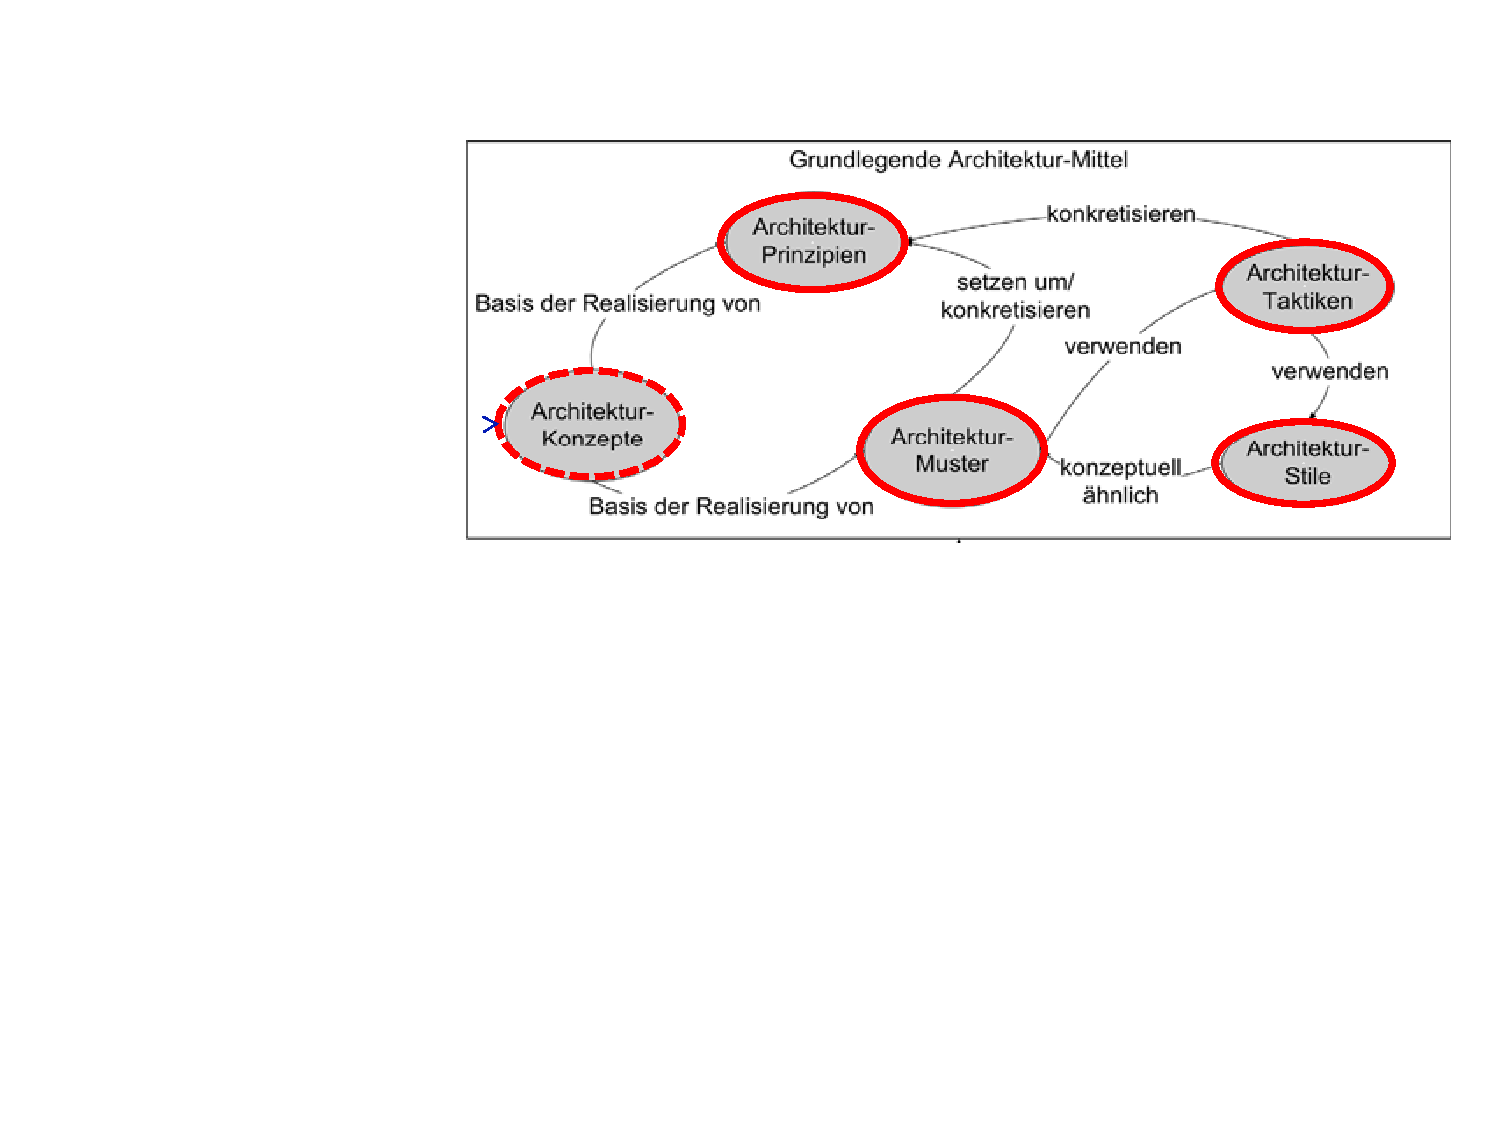
\includegraphics[width=0.7\linewidth]{fig/begriffe}
\caption{Grundlegende Begriffe}
\label{fig:begriffe}
\end{figure}

Bei einem Architekturentwurf werden Anforderungen, Qualitätsmerkmale und Rahmenbedingungen in den Prozess hineingegeben und heraus kommt eine Architektur welche durchführbar und entwicklungsfähig ist. Um so eine Architektur hinzukriegen, werden die Methoden in Abbildung \ref{fig:begriffe} angewendet. Abbildung \ref{fig:twin-peaks} zeigt das erweitere Twin Peaks Modell. Es soll aufzeigen dass die Architektur der Vermittler zwischen Anforderungen und Konstruktion ist. Zudem wird das ganze System in einem iterativen Prozess entworfen, was die Spirale darstellen soll.

\begin{figure}
\centering
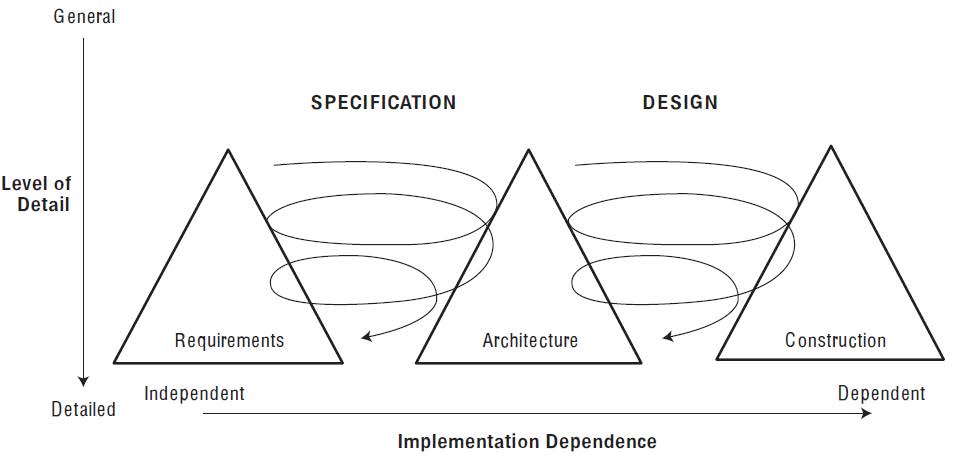
\includegraphics[width=0.7\linewidth]{fig/twin-peaks}
\caption{Erweitertes Twin Peaks Modell}
\label{fig:twin-peaks}
\end{figure}

Der iterative, inkrementelle Prozess des Architekturentwurfs läuft immer gleich ab:
\begin{enumerate}
	\item Analyse der Anforderungen und Auflösung von Konflikten
	\item Anwendung von Prinzipien, Taktiken \& Mustern
	\item Treffen von Entscheidungen \& Kompromissen
	\item Bewertung von Alternativen
	\item Bereitstellen von Sichten für Beteiligte
	\item Dokumentation und Bewertung von Entscheidungen
	\item Wenn Entwurf ok umsetzen sonst \verb|goto 1|
\end{enumerate}
Zum Schluss: Jedes System hat eine Architektur auch wenn keine Beschreibung ausserhalb des Codes existiert und sie in der Implementierung schwer zu erkennen ist.

\section{Funktionale Anforderungen: Use cases und User Stories}

\section{Nichtfunktionale Anforderungen: Szenarios 
Prinzipien \& Taktiken}

\section{Stile und Muster}

\section{Sichten, Architekturentscheidungen und Dokumentation}

\section{Bewertung von Architekturen (ATAM)}

\section{Beruf des IT Architekten}

\section{Fallstudie Fillialbestellsystem aus Modul Applikationsentwicklung}